% Be more explicit about outlining what this section will do/show and guide the reader so they know what to expect.
In this section, we introduce a unified system of equations 
to describe risk group dynamics %make sure 'risk group dynamics' is clearly defined in the introduction
in deterministic epidemic models with heterogeneity in risk.
We then describe how the unified approach can be used in practical terms based on 
different assumptions and different data available for parameterizing risk group dynamics or turnover in risk. % use one or the other terminology as much as possible
We conclude by framing our approach in the context of approaches used in previous models of HIV/STI transmission. % if STI transmission models included in the prior literature part
% ==================================================================================================
\subsection{Notation}
Consider a population divided into $G$ risk groups.
The number of individuals in risk group $i \in [1, \dots, G]$ is denoted as $x_i$
and the set of all risk groups is denoted as $\bm{x} = \{x_1, \dots, x_G\}$.
The total population size is $N = \sum_i {x_i}$,%
\footnote{Here, as in many models, ``total population'' actually represents  %suggest removing this footnote. Not relevant here and distracts from discussion of subsets in the context of the modeled population subgroups
  a subset of the population with a consistent duration in the model --
  e.g. an age-constrained range.}
  
and the relative population size of each group 
is denoted as $\hat{x}_i = x_i / N$.
Individuals enter the modeled system at a rate $\nu$ per year,  %in the system section, suggest calling it a 'system' or 'modeled system' rather than the model since the model in the later section refers to the SIR system?  The term 'exogenous' can refer to entering from outside; vs. endogenous entry which refers to turnover. As you know I do not like new terms but we may need these two terms which are commonly used in science - as long as we define them.

and exit at a rate $\mu$ per year. We refer to this as exogenous entry/exit as it refers to how individuals enter and leave the modeled population.
The proportion of all individuals who exogenously enter group $i$ 
may be different from
the proportion of individuals currently in group $i$ in the model ($\hat{x}_i$). % say why they may be different? currently reads as though the reader will already know why

Therefore, we distinguish these proportions %suggest avoiding saying 'these' and best to repeat what you mean by 'these proportions' - e.g. we distinguish between the proportion who enter and the proportion currently in group $i$, and denote the former as ...
and denote the proportion entering into group $i$ as $\hat{e}_i$.
For example, a higher proportion of youth (model entrants, $\hat{e}_i$)    %i could not follow this sentence - needs to be rephrased for clarity
may engage in high-risk sexual behaviour,
as compared to the population overall ($\hat{x}_i$).
In section XXX we demonstrate 
how rates of turnover can maintain such a system at equilibrium.  % (1) where will it be shown? if saying later or 'above', etc. -- give a bookmark to guide the reader. (2) Why do we need to keep the system at equilibrium? The concept of maintaining the system at equilibrium has not been introduced in intro I think...; (3) also ensure that the term 'turnover' has already been introduced and defined earlier.

%The number of entrants into group $i$ is therefore given by
%$\nu N \hat{e}_i$.
%This assumption then implies then implies the existence of
%a ``source'' population $\bm{e} = \{e_1, \dots, e_G\}$,
%from which model entrants originate.
%The size of this population is then assumed to be the same as $\bm{x}$ ($\sum_i e_i = N$)
%so that the entry rate $\nu$ can be used in the usual way,
%as a proportion of $N$.
\par
Turnover transitions can occur between any two groups and in either direction such %beware overuse of semi-colons
that turnover rates can be denoted as a $G \times G$ matrix $\phi$.
The element $\phi_{ij}$ corresponds to the proportion of individuals in group $x_i$
who move from group $x_i$ to group $x_j$ each year.
An example matrix is given in Eq.~(\ref{eq:phi}),
where the diagonal elements are written $*$ since they represent
transitions from a group to itself and thus, are not relevant. % inconsequently suggests they can still occur? 
\begin{equation}\label{eq:phi}
\phi = \left[\begin{array}{cccc}
	         *          & x_1  \rightarrow x_2 & \cdots & x_1 \rightarrow x_G \\[0.5em]
	x_2 \rightarrow x_1 &          *           & \cdots & x_2 \rightarrow x_G \\[0.5em]
	      \vdots        &        \vdots        & \ddots &       \vdots        \\[0.5em]
	x_G \rightarrow x_1 & x_G \rightarrow x_2  & \cdots &          *
\end{array}\right]
\end{equation}
These transitions and their associated rates		%transitions and flows say the same thing, so I think ok to use one term
are shown for $G = 3$ in Figure~\ref{fig:system}.
\begin{figure}
  \centering
  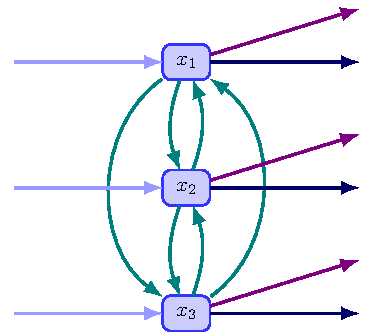
\includegraphics[width=0.5\linewidth]{turnover-system}
  \caption{System of states and flows between them for $G = 3$}
  \label{fig:system}
\end{figure}
% ==================================================================================================
\subsection{Parameterization}\label{ss:params}
We now construct a system 
to reflect the risk group dynamics observed in a real-world context.  %later make sure to do a consistency check for terminology
% do you mean using real-world data? that might be preferred here instead of real-world context since talking about specific parameters and not 'everything'?
We begin with the assumption 
that the number of risk groups included in the model has already been defined,
and that the relative population sizes of these groups ($\hat{x}_i$) should remain constant over time. %important to discuss re: generalizability in the Discussion section; and esp when highlighting the limitation of use with HIV which has important disease-attributable mortality.
Thus, the following parameters must be estimated using available data:
$\nu$, $\mu$, $\bm{\hat{x}}$, $\bm{\hat{e}}$, and $\phi$.
% --------------------------------------------------------------------------------------------------
\subsubsection{Total Population Size}\label{sss:params-nu-mu}
The difference between the entry rate $\nu(t)$ and exit rate $\mu(t)$ for a population,
gives a net growth rate $\mathcal{G}(t)$.
The total population $N(t)$ is then defined by the exponential growth
of the original population $N_0$ according to $\mathcal{G}(t)$,
% TODO: this is not trivial!
\begin{subequations}
  \begin{align}
  \mathcal{G}(t) &= \nu(t) - \mu(t)            \label{eq:growth-G}\\
%  N(t) &= N_0 \prod_{\tau}^{t} \big(1+\mathcal{G}(\tau)\big) \label{eq:growth-N}
  \end{align}
\end{subequations}
Note that the average duration of an individual in the model at time $t$ is given by:
\begin{equation} \label{eq:duration-model}
\delta(t) = \mu^{-1}(t)
\end{equation}
Variation in rate of entry across risk groups is captured in $\bm{\hat{e}}$,
and rate of exit is generally not stratified by activity group
(besides disease-attributable death, which we do not consider here).
Therefore, it can be assumed that $\nu$ and $\mu$ do not vary across risk groups,
allowing these rates to be derived independent of
the population proportions $\bm{\hat{x}}$, $\bm{\hat{e}}$, and turnover $\phi$.
\par
The simplest approach to obtaining $\nu$ and $\mu$ assumes
a constant population size $N(t) = N_0$.
This implies a growth rate of zero, yielding $\nu = \mu$.
However, this does not reflect the positive population growth of most real contexts.
%and may result in underestimated incidence,
%due to the relative reduction in inflow of susceptible individuals.
% verified in code, see:
% https://github.com/c-uhs/turnover/blob/f029bd1/outputs/figs/debug/incidence-nu.gif
% \cite{} ?
Another approach is to fix $\mathcal{G}(t)$ as some constant.
When using this approach, care should be taken to ensure
the resulting $N(t)$ matches available population size estimates to a reasonable degree.
\par
Typically, data will be available for the total size of the population over time $N(t)$,
so the growth rate for each time interval $t_i$
can be derived by rearranging Eq.~(\ref{eq:growth-N}):
\begin{equation}
\mathcal{G}(t_i) = {\left(\frac{N(t_{i+1})}{N(t_{i})}\right)}^{-(t_{i+1}-t_i)} - 1
\end{equation}
All of these approaches help define $\mathcal{G}(t)$, but leave one degree of freedom,
since many choices of $\mu(t)$ can be compensated by an appropriate choice of $\nu(t)$
to yield the desired $\mathcal{G}(t)$.
However, an assumed duration of individuals in the model $\delta(t)$
can usually be leveraged to choose $\mu(t)$ as in Eq.~(\ref{eq:duration-model}).
This duration can be assumed,
or be chosen to reflect the age range in data sources for other model parameters.
Then, $\nu(t)$ can be resolved using the growth rate in Eq.~(\ref{eq:growth-G}).
% --------------------------------------------------------------------------------------------------
\subsubsection{Turnover}\label{sss:params-turnover}
% TODO: discuss common approaches - especially turnover is constant, or zero.
% TODO: discuss more the assumptions throughout.
% TODO: add approach for balancing absolute flows between compartments
Next, methods for resolving $\bm{\hat{e}}(t)$ and $\phi(t)$
are presented, assuming that $\nu(t)$ and $\mu(t)$ are known.
Similar to above, the problem is first formulated as a system of equations.
then the data and assumptions which can be leveraged to solve the system will be considered.
\par
We begin by defining the ``conservation of mass'' equation for a given group $x_i$,
where that the rate of change of the group
is simply the sum of flows in~/~out of the group:
\begin{equation}\label{eq:mass-balance}
\frac{d}{dt}x_i
= \nu \thinspace e_i + \sum_{j}{\phi_{ji} \thinspace x_j}
- \mu \thinspace x_i - \sum_{j}{\phi_{ij} \thinspace x_i}
\end{equation}
While Eq.~(\ref{eq:mass-balance}) is written in terms of
absolute population sizes $\bm{x}$ and $\bm{e}$,
it is equivalent to divide through by $N$, yielding a system in terms of
proportions $\bm{\hat{x}}$ and $\bm{\hat{e}}$,
which is often more useful, since $N$ need not be known.
\par
We further assume that the average proportions of each group $\hat{x}_i$ do not change over time.
Therefore, the desired rate of change for risk group $i$
will be equal to the growth of the risk group, $\mathcal{G} x_i$.
Substituting this into Eq.~(\ref{eq:mass-balance}),
and simplifying, we have:
\begin{equation}\label{eq:system}
\nu \thinspace x_i
= \nu \thinspace e_i + \sum_{j}{\phi_{ji} \thinspace x_j}
- \sum_{j}{\phi_{ij} \thinspace x_i}
\end{equation}
Now, depending on the number of risk groups, we have
$G$ and $G(G-1)$ unknowns in $\bm{e}$ and $\phi$, totalling $G^2$ variables to resolve.
We denote these variables as the vector $\bm{\theta} = \left[\bm{e}, \bm{z}\right]$,
where $\bm{z} = \mathrm{vec}_{i \ne j}(\phi)$;
this allows us to define
a system of linear equations of the form:
\begin{equation}\label{eq:system-matrix}
\bm{b} = A \thinspace \bm{\theta}
\end{equation}
where $A$ is a $G \times G^2 $ matrix
and $\bm{b}$ is a $G$-length vector,
representing the right-hand side and left-hand side of Eq.~(\ref{eq:system}), respectively.
In this form, we can use $A^{-1}\bm{b} = \bm{\theta}$ to solve for $\bm{\theta}$.
\par % TODO: underdetermined by this? What about sum{e} = 1?
Unfortunately, for any $G > 1$, the system is underdetermined by a factor of $G(G-1)$,
meaning there are many combinations of $\bm{e}$ and $\phi$ which satisfy Eq.~(\ref{eq:system}).
Therefore, we now resume our task of leveraging data and assumptions
to define a unique solution.
\par
Our first tool is another equation.
We note that the duration of time spent in a particular group $\delta_i$
is the inverse of all efferent flow rates:
\begin{equation}\label{eq:duration-group}
\delta_i = {\bigg(\mu + \sum_{j}{\phi_{ij}}\bigg)}^{-1}
\end{equation}
These durations could be derived from survey data, including for key populations,
or they could be assumed.
Rearranging Eq.~(\ref{eq:duration-group}), we obtain
${\delta_i}^{-1} - \mu = \sum_{j}{\phi_{ij}}$,
which yields an additional $G$ equations in our linear system -- i.e.\ rows of $A$ and $\bm{b}$.
For $G = 2$, this provides enough constraints to fully determine the system, % TODO: does it though? as 2nd duration is redundant, no?
as shown in \ref{aa:eqs-turnover} \nameref{aa:eqs-turnover},
but for larger $G$, still more constraints are needed.
\par
The simplest additional constraints can be elements in $\bm{\theta}$ which are directly specified
-- i.e.\ elements of of $\bm{e}$ or $\phi$.
For example, the proportion of individuals who
move from one risk group to another each year ($\phi_{ij}$)
may be assumed or derived from data.
Similarly, the distribution of individuals
across risk groups in the entering population $\bm{\hat{e}}$
may be approximated using the proportions among
the lowest age group for which data are available.
In each case, the value specified is appended to $\bm{b}$,
and a row appended to $A$ of the form: $[0,\dots,1,\dots,0]$,
with $1$ in the position of the element in $\bm{\theta}$.
\par
There are, however, two notable caveats to this approach.
First, not all combinations of specified elements will add an equal number of constraints.
Specifying all elements of $\bm{e}$
will only add $G-1$ (not $G$) constraints,
since $\sum \bm{\hat{e}} = 1$, so the final element adds no new information.
Similarly, specifying all elements of $\phi_{ij}$ for a given $i$
as well as the duration for the group $\delta_i$
will only add $G-1$ (not $G$) constraints,
since Eq.~(\ref{eq:duration-group}) must hold.
%\footnote{Recall that the diagonal elements of $\phi$ are inconsequential,
%  so only $G-1$ elements of $\phi_{ij}$ may be specified at all for a given $i$.}
Second, not all combinations of specified values will yield a valid solution,%
\footnote{Even rank-deficient systems be inconsistent.}
and it is unfortunately difficult to anticipate problematic combinations.
\par
Finally, we note that additional constraints may be avoided altogether if we pose the problem
as an optimization problem, namely:
\begin{equation}\label{eq:system-optimize}
\bm{\theta}^{*} = {\arg \min}
\thinspace f(\bm{\theta}),
\quad \textrm{subject to:}
\enspace\bm{b} = A\thinspace\bm{\theta};
\enspace\bm{\theta} \ge 0
\end{equation}
where $f$ is a function such as ${\left|\left| \thinspace\cdot\thinspace \right|\right|}_2$.
However, the choice of $f$ implies a prior on the values of $\bm{\theta}$,
and so introduces bias in the solution.
% ==================================================================================================
\subsection{Previous Approaches}
INP
\begin{floatbox}
  \caption{Common assumptions regarding the dynamics of risk groups}
  \label{box:assumptions}
  \begin{fboxed}
  \begin{enumerate}[leftmargin=1em]
    \item\label{ass:risk-groups}\textbf{Risk Groups:}
    Major demographic groups are stratified by risk of HIV acquisition.
    \begin{enumerate}
      \item\label{ass:risk-groups-no}\textbf{No:} $\G = 1$;
      Major demographic groups are homogeneous in risk of HIV acquisition.
      \item\label{ass:risk-groups-yes}\textbf{Yes:} $\G > 1$;
      Heterogeneity in risk of HIV acquisition within major demographic groups is considered.
    \end{enumerate}
    \item\label{ass:turnover}\textbf{Turnover:}
    Individuals may move between risk groups.
    \begin{enumerate}
      \item\textbf{No:} $\zeta = 0$;
      Individuals do not move between risk groups.
      \item\textbf{Constant:} $\zeta > 0$;
      Individuals move between risk groups at a constant rate.
%      \item\textbf{Dynamic:} $\zeta = f$;
%      Individuals move between risk groups in dynamically.
    \end{enumerate}
    \item\label{ass:pop-growth}\textbf{Population Growth:}
    Increase in the total $\N$ over time.
    \begin{enumerate}
      \item\textbf{No:} $\nu = \mu$;
      Population size $\N$ is constant.
      \item\textbf{Yes:} $\nu > \mu$;
      Population size $\N$ increases, at some constant or data-driven rate.
    \end{enumerate}
  \end{enumerate}
\end{fboxed}

\end{floatbox}

